\chapter{Kuhn poker experiment} \label{PLEI}

\lhead{Chapter x. \emph{Kuhn poker experiment}}
In this chapter we will present and explain the experiment on a simplified version of poker, the Kuhn poker.
Fist we will describe how we setup the neural network and how we trained it. Then we will present the result and the different metrics on how good the neural network performed. Finally we will analyze the result and try to generalize them to any imperfect game.

\section{Setup} \label{kuhnexperiment:setup}

\subsubsection{environment}
We created a Kuhn poker environment which give us all the necessary data to correctly feed the neural network. We have defined 3 actions possible: check, bet and fold. We have decided to regroup raise and bet in a same action "bet" to reduce the complexity. If at any time the decision making NN predict an incorrect action, the default action "bet" or "check" would be done.

\subsubsection{NN}
We decided to first use a simple RNN for the opponent modelling, you can find more information about the specific input of this NN in section \ref{methodology:opponent-modelling}, see figure \ref{fig:opponent-modelling-nn-rnn}. We used the decision making NN describe in section \ref{methodology:descision-making}, figure \ref{fig:decision-making-nn}. Different layers, activation function and opponent model size has been tested. Only the most successful architecture will be presented, their results will be detailed in the section \ref{kuhnexperiment:result}. The descriptions of the NN layers are detailed in table \ref{tab:nn-layer-kuhn}.

\begin{table}[ht]
\begin{tabular}{ |c|c|c| }
 \hline
 NN name & opponent-modelling NN  & descision-making NN \\ 
 \hline
 input layer & x & x \\ 
 \hline
 hidden layer & 10 & 10 \\
 activation & linear & linear \\
 \hline
 output layer & opponent model size & 3 (check, bet, fold) \\
 activation & linear & softmax \\
 \hline
\end{tabular}
\caption{NN layer (kuhn poker)}
\label{tab:nn-layer-kuhn}
\end{table}

The size of the input layer is defined by the environment and the opponent model size. It has been detailed in the section \ref{methodology:NN}. 

\subsection{Training}
To train the NN we have used competitive co-evolution, general information about it can be found in section \ref{methodology:competitive-co-evolution}.

We have used these strategy in the teaching set:

\begin{itemize}
    \item \textbf{Equilibrium}: playing the equilibrium strategy
    \item \textbf{Random}: playing a random action in the set of the available ones
    \item \textbf{Always bet}
    \item \textbf{Always fold}
    \item \textbf{Close Equilibrium}: playing a strategy close to the equilibrium. It select each action with a probability chosen uniformly randomly within 0.2 of the equilibrium probability. It aims to produce realistic sub-optimal opponent.
\end{itemize}

We have by default added 3 different \textit{Close Equilibrium} strategy to the teaching set.

We have not used a system to dynamically add training agents to the teaching set.

We are making each agents playing against each other and using a shared fitness to promote diversity (ref: \ref{LR:competitive-co-evolution}). To make the result of the games not based on cards luck, we are first making the two agents play a set of round. Then, we erase their memory and make them play with the opposite cards. A temporary reward is attributed, the agent winning 1, the one loosing -1, then the final reward is attributed after the shared fitness calculation.

The EA has been used with these parameters:
\begin{itemize}
    \item population size: 20
    \item individual kept each iteration: 5
    \item mutation rate: 0.1
    \item iteration: 100
    \item number of rounds (games): 25
\end{itemize}

These parameters has been decided after multiple iterations, those seems to have good training performance in this context.

\section{Result} \label{kuhnexperiment:result}
In order to evaluate the NN we apply the evaluation method detailed in the section \ref{requirement:evaluation}.

In this section, results of multiple NN models will be presented, the NN and EA paremeters are by default the one described in the previous section \ref{kuhnexperiment:setup}.

\begin{itemize}
    \item \textbf{Classic}: No parameters changes.
    \item \textbf{More Games}: Playing 50 games per iteration (instead of 25). Only 10 individuals and 3 are kept at each iteration.
    \item \textbf{Bigger Model Size}: The opponent model size is 10 (instead of 5)
    \item \textbf{Larger Teaching Set}: Having 6 \textit{Close Equilibrium} agents in the teaching set
\end{itemize}

\subsection{Win rate}

In this section we will present the win rate of the different tested models against multiple strategy, the choices of the strategy is detailed in the section \ref{requirement:evaluation}. You can find the results in the table \ref{tab:reward-kuhn} (Equilibrium has been shorten to E and true best response to TBR).

\begin{table}[h]
\begin{tabularx}{\textwidth}{ |c|X|X|X|X|X|X|X| }
 \hline
 Opponent Model & E & Close E & Random & Always Bet & Always Fold & TBR & Random then TBR \\ 
 \hline
 Classic & 0.001 & 0.053 & 0.202 & 0.293 & 0 & -0.182 & -0.139 \\
 \hline
 More Games & 0.006 & 0.001 & 0.312 & 0.200 & 0.646 & -0.175 & -0.116 \\ 
 \hline
 Bigger Model Size & -0.02 & 0.027 & 0.309 & 0.180 & 0.106 & -0.087 & -0.065 \\
 \hline
 Larger Teaching Set & 0.001 & 0.054 & 0.196 & 0.350 & 0 & -0.172 & -0.120 \\
 \hline
 Equilibrium & 0 & 0.007 & 0.150 & 0.104 & 0.238 & -0.125 & -0.118 \\
 \hline
\end{tabularx}
\caption{Win rate in mbb/hand of the opponent model against evaluation opponent (kuhn poker)}
\label{tab:reward-kuhn}
\end{table}

We can see that the model \textbf{A} and \textbf{B} have really good performance against the exploitable strategy such as Always Bet, Always Fold and Random. Compared to the equilibrium their final reward is at least doubled. However the model \textbf{B} is more exploitable than model \textbf{A} as demonstrate the reward against equilibrium and best response.

The main difference between the model \textbf{A} and \textbf{B} is that \textbf{A} is way more resistant to exploitation. Indeed, the model \textbf{A} is capable of exploiting some strategy without sacrificing performance against strong strategy such as Equilibrium or best response.

% FLASE It is worth to mention that model \textbf{A} perform poorly against always fold, an opponent that is supposed to be easily exploitable. We can assume it is linked to the way NN are trained. In competitive EA with shared fitness, it is likely that a strategy exploiting a stronger opponent (always bet) will have a better fitness that other exploiting a simple opponent (always fold).


\subsection{Reward over time}

In this section we will present the interesting plots of the reward over time for different model.

The different plots showcase on this section are based on 1000 played games. It is worth to note that the EA training has been run having only 25 games played between each agent. Using a different scale (from 25 to 1000) demonstrate how the NN model handle keeping an opponent model throught more game than usual.

\begin{figure}[ht]
    \centering
    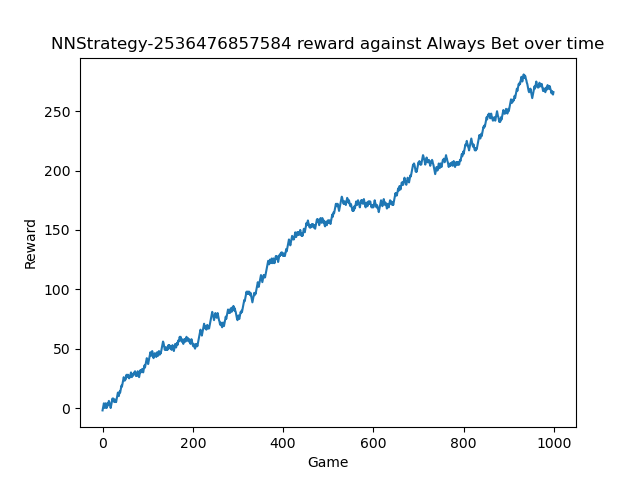
\includegraphics[width=0.7\textwidth]{Figures/out-plots/kuhn/B/reward-against-Always Bet.png}
    \caption{Model B, reward against Always Bet over time}
    \label{fig:kuhn:b-always-bet}
\end{figure}

In figure \ref{fig:kuhn:b-always-bet}, you can see that at the very beginning, the reward is neither increasing or decreasing. Then after some games, we can assume that the NN draw a model of the opponent, and start to exploit it by having a relatively stable increasing of the reward.

\begin{figure}[ht]
    \centering
    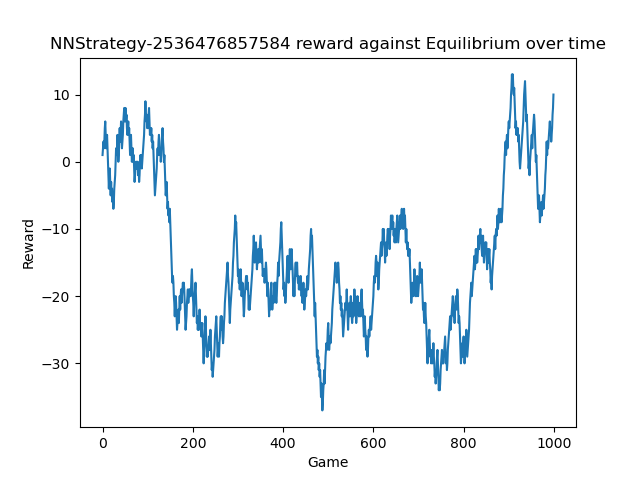
\includegraphics[width=0.7\textwidth]{Figures/out-plots/kuhn/B/reward-against-Equilibrium.png}
    \caption{Model B, reward against Equilibrium over time}
    \label{fig:kuhn:b-equilibrium}
\end{figure}

In figure \ref{fig:kuhn:b-equilibrium}, you can see that there is not a straight tendency of increasing or decreasing. It's somehow what you except from a game against two opponents without a net exploitation. It demonstrate the ability of the model to not fall into a wrong interpretation, or at least recover / correct the opponent model.

% TODO graph and analysis

\subsection{Input impact on the NN} \label{kuhnexperiment:result:input-impact}

We have measured the impact of each input to every output of the neural network to determine how much the input is take in consideration in the decision. In order to do that we used SHAP \citep{shap}, a game theoretic approach to explain the output of any machine learning model.

The inputs are ordered by impact. Each blue dot represent the impact (positive or negative) of an input for one activation.

\begin{figure}[ht]
    \centering
    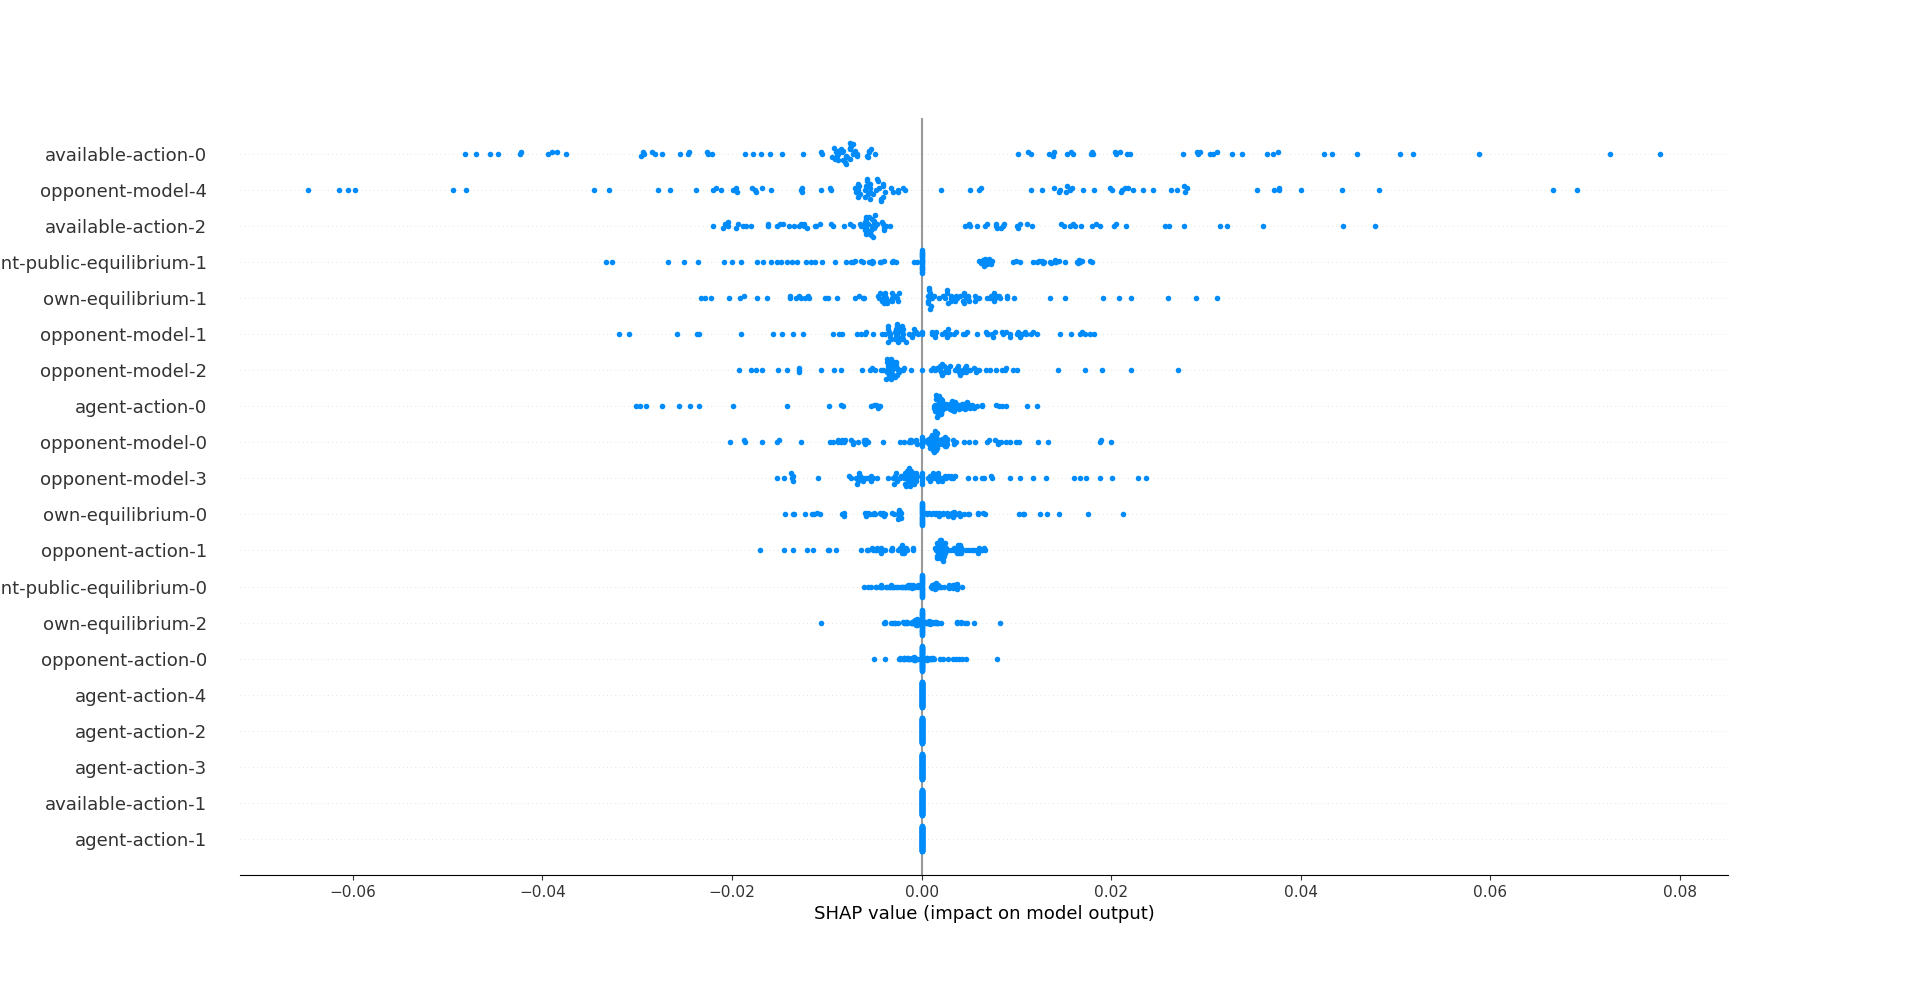
\includegraphics[width=1\textwidth]{Figures/out-plots/kuhn/A/action-check-input-impact.png}
    \caption{Model A, input impact for the check action}
    \label{fig:kuhn:a-impact-check}
\end{figure}

On the figure \ref{fig:kuhn:a-impact-check} (check), we can see the input \textit{opponent-model-4} is the second input with the most impact on the decision if either he should check or not. In addition \textbf{opponent-model-1} and \textbf{opponent-model-2} are the 6th and 7th most impacting input. It demonstrate that the NN highly rely on the opponent model to take its decision.

\begin{figure}[ht]
    \centering
    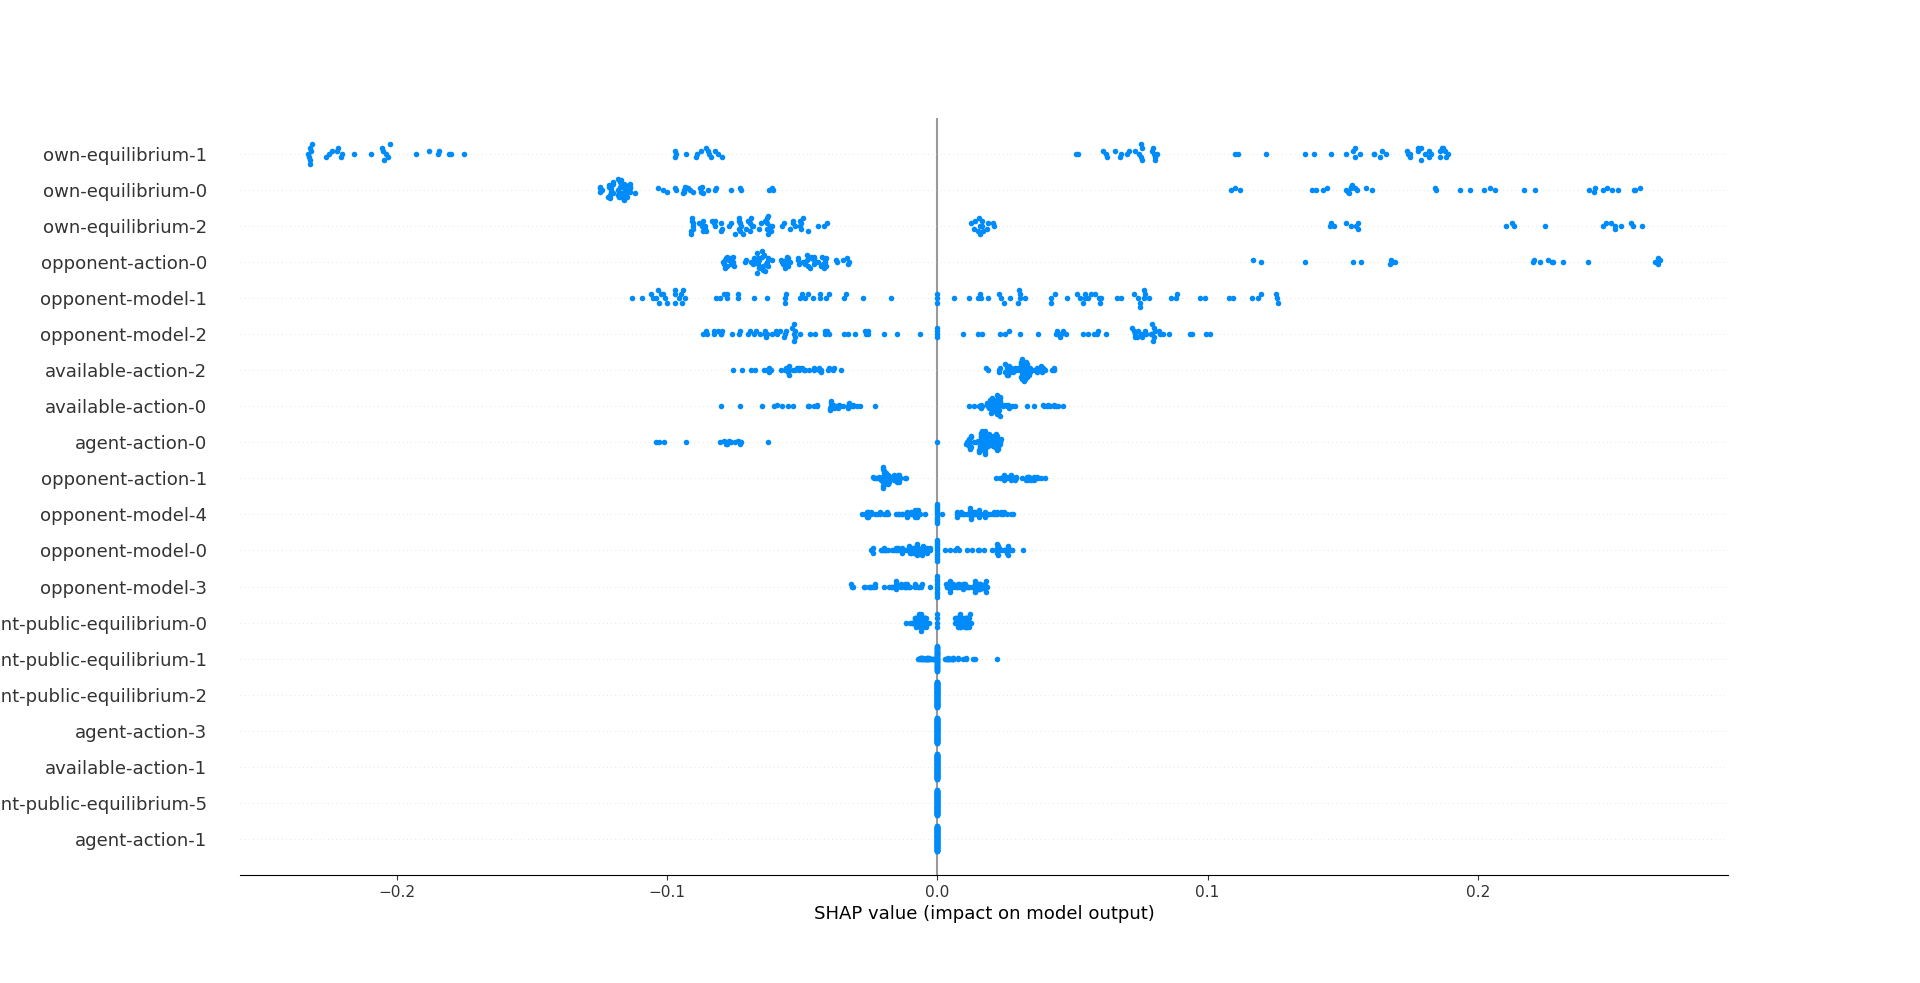
\includegraphics[width=1\textwidth]{Figures/out-plots/kuhn/A/action-fold-input-impact.png}
    \caption{Model A, input impact for the fold action}
    \label{fig:kuhn:a-impact-fold}
\end{figure}

On the figure \ref{fig:kuhn:a-impact-fold} (fold), we can see that it rely way more on the equilibrium as they represent the three most impacting input. The opponent model still have an important place, indeed \textbf{opponent-model-1} and \textbf{opponent-model-2} are the 5th and 6th most important input.

Comparing the figure \ref{fig:kuhn:a-impact-check} (check) and the figure \ref{fig:kuhn:a-impact-fold} (fold), we can see that the \textbf{opponent-model-4} input has only a real impact for the action check. This means that a part of the opponent model is specialized for a specific action.

% TODO opponent model 4 which input impact it

\subsection{Best response}

The best response help understand how much an algorithm is exploitable, it have access to every player cards and play the best response every-time. It is not an absolute metric but highlight if an algorithm is likely to be exploitable.

The best response result are presented in this table \ref{tab:reward-over-time-kuhn}

\section{Analysis and generalisation}

\subsection{Opponent model specialisation}

We have seen in the section \ref{kuhnexperiment:result:input-impact} that a part of the opponent model has been specialized for a specific action. Such a specialisation underline the importance in opponent exploitation to link the opponent modeling and decision making training. Indeed to develop a specialisation the opponent model needs to match the decision making needs and I believe that this process can reach his full potential only during the training phase.

\subsection{Approximation or incorrect Equilibrium}

During the development, I had a bug that allowed cards to be draw multiple times. For example it was possible to have the player one king and the second with an other king (which is not possible in the kuhn poker). So it mades the equilibrium incorrect. In the figure TODO you can see that even if the equilibrium was incorrect it managed to overcome this and exploit the different strategies. This means that using NN to exploit opponent in imperfect game using this NN architecture can manage and overcome incorrect or approximated equilibrium.

It is worth to mention that the performance are likely to be degraded because the NN will need to learn the game. Indeed it will likely rely on the game history such as the previous action instead of relying on the equilibrium.